\documentclass[11pt]{article}
\usepackage[paperwidth=13.333in,paperheight=7.5in,margin=0.25in]{geometry}
\pagestyle{empty}
\usepackage{tikz}
\usetikzlibrary{arrows.meta,positioning,fit,calc,shapes.geometric,backgrounds}
\usepackage{xcolor}
% The default palette is the white-background evidence-report style. The
% figure builder defines \DARKTHEME for slide-ready variants.
\ifdefined\DARKTHEME
\definecolor{ink}{HTML}{F3F7FA}
\definecolor{muted}{HTML}{B9C7D4}
\definecolor{grid}{HTML}{2B3B4B}
\definecolor{blue}{HTML}{62B8FF}
\definecolor{teal}{HTML}{55D6C2}
\definecolor{orange}{HTML}{FFBD5A}
\definecolor{red}{HTML}{FF7568}
\definecolor{purple}{HTML}{C3A6FF}
\definecolor{paleBlue}{HTML}{14283A}
\definecolor{paleOrange}{HTML}{3A2B14}
\definecolor{dataFill}{HTML}{241C3A}
\definecolor{modelFill}{HTML}{12352F}
\definecolor{specialistFill}{HTML}{3A2B14}
\definecolor{futureFill}{HTML}{1C2630}
\definecolor{pageBg}{HTML}{080D13}
\else
\definecolor{ink}{HTML}{102A43}
\definecolor{muted}{HTML}{52606D}
\definecolor{grid}{HTML}{D9E2EC}
\definecolor{blue}{HTML}{1976A8}
\definecolor{teal}{HTML}{16817A}
\definecolor{orange}{HTML}{D9822B}
\definecolor{red}{HTML}{C05640}
\definecolor{purple}{HTML}{6B5B95}
\definecolor{paleBlue}{HTML}{E8F1F5}
\definecolor{paleOrange}{HTML}{FFF1DF}
\definecolor{dataFill}{HTML}{F5F0FA}
\definecolor{modelFill}{HTML}{EAF6F4}
\definecolor{specialistFill}{HTML}{FFF1DF}
\definecolor{futureFill}{HTML}{F2F4F5}
\definecolor{pageBg}{HTML}{FFFFFF}
\fi
\pagecolor{pageBg}
\tikzset{
  base/.style={font=\sffamily, text=ink},
  title/.style={base, font=\sffamily\bfseries\fontsize{23}{27}\selectfont},
  subtitle/.style={base, font=\sffamily\fontsize{12}{15}\selectfont, text=muted},
  box/.style={base, rounded corners=3pt, draw=blue!65!black, fill=paleBlue, minimum height=0.78cm, minimum width=2.65cm, align=center, inner sep=7pt},
  data/.style={box, draw=purple!75!black, fill=dataFill},
  model/.style={box, draw=teal!75!black, fill=modelFill},
  specialist/.style={box, draw=orange!85!black, fill=specialistFill},
  future/.style={box, draw=muted, fill=futureFill, dashed},
  arrow/.style={-{Latex[length=3mm]}, line width=0.9pt, draw=muted},
  dashedarrow/.style={-{Latex[length=3mm]}, line width=0.8pt, draw=muted, dashed},
  note/.style={base, font=\sffamily\fontsize{18}{22}\selectfont, text=muted, align=left},
}

\begin{document}
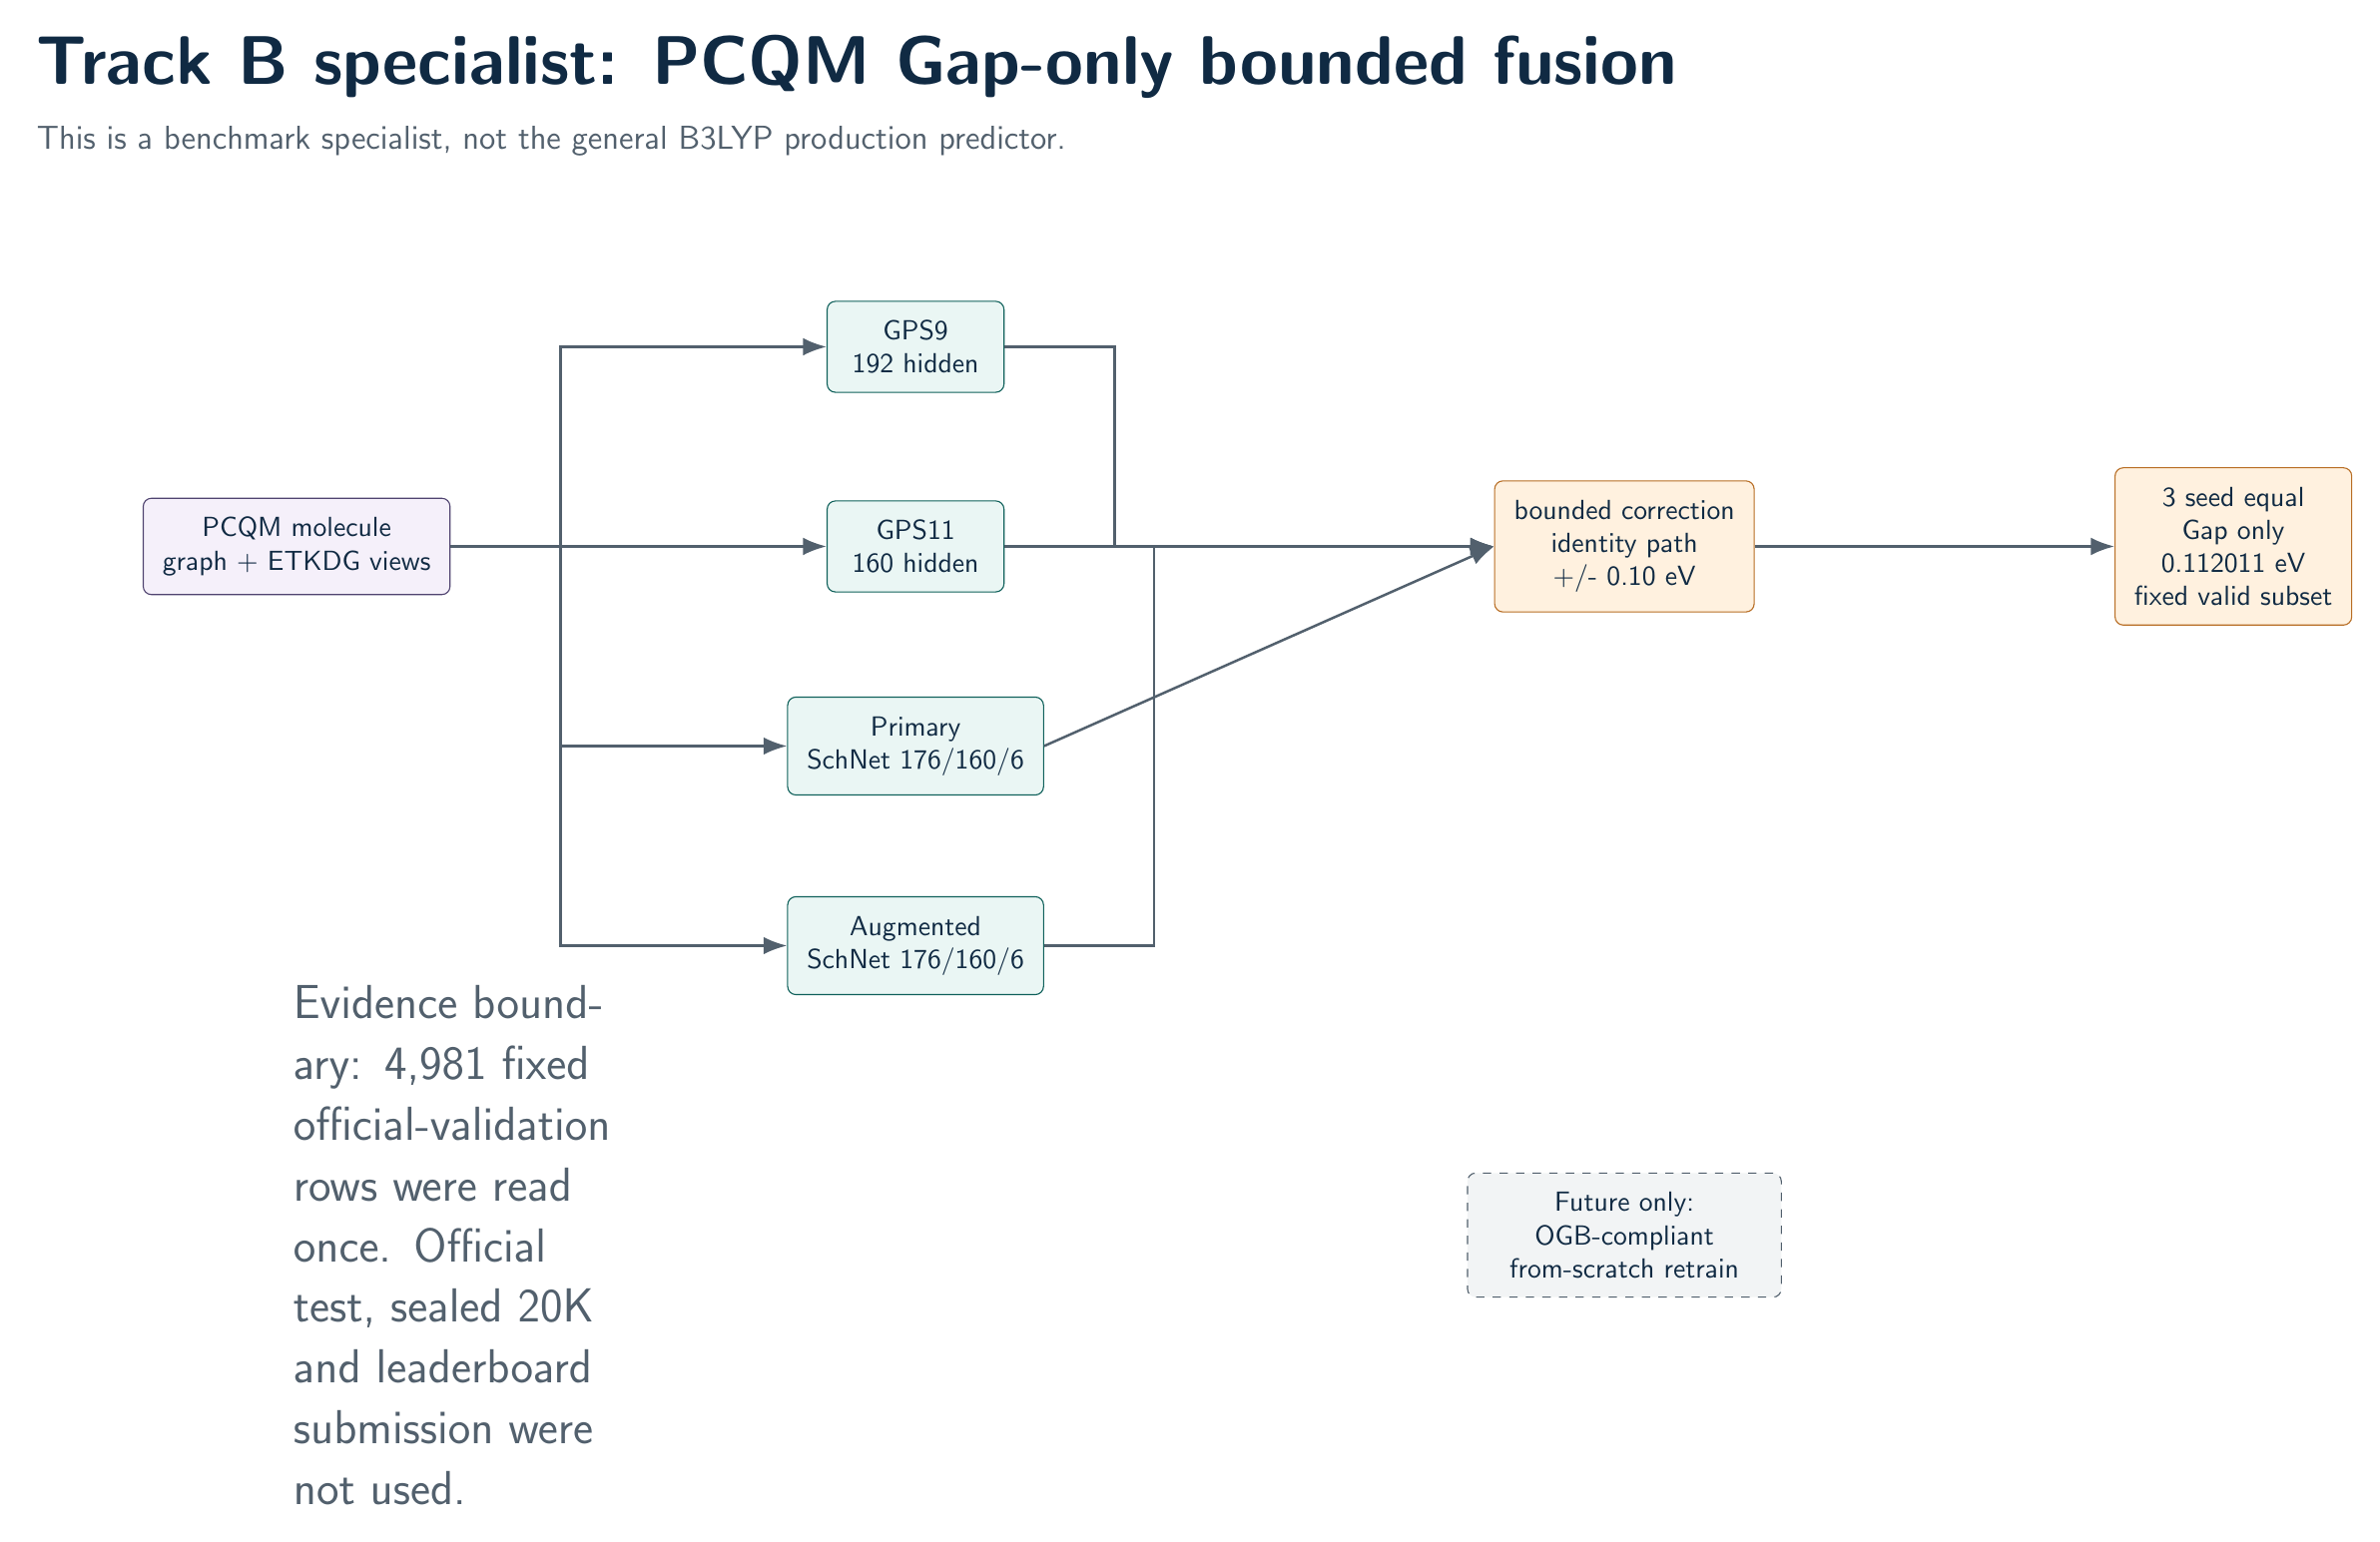
\begin{tikzpicture}[x=1in,y=1in]
  \node[title,anchor=west] at (0,6.85) {Track B specialist: PCQM Gap-only bounded fusion};
  \node[subtitle,anchor=west] at (0,6.48) {This is a benchmark specialist, not the general B3LYP production predictor.};

  \node[data,minimum width=2.65cm,minimum height=1.0cm] (input) at (1.35,4.45) {PCQM molecule\\graph + ETKDG views};
  \node[model,minimum width=2.25cm,minimum height=0.95cm] (g9) at (4.45,5.45) {GPS9\\192 hidden};
  \node[model,minimum width=2.25cm,minimum height=0.95cm] (g11) at (4.45,4.45) {GPS11\\160 hidden};
  \node[model,minimum width=2.25cm,minimum height=0.95cm] (s1) at (4.45,3.45) {Primary\\SchNet 176/160/6};
  \node[model,minimum width=2.25cm,minimum height=0.95cm] (s2) at (4.45,2.45) {Augmented\\SchNet 176/160/6};
  \node[specialist,minimum width=2.75cm,minimum height=1.15cm] (fusion) at (8.0,4.45) {bounded correction\\identity path\\+/- 0.10 eV};
  \node[specialist,minimum width=2.7cm,minimum height=1.15cm] (ens) at (11.05,4.45) {3 seed equal\\Gap only\\0.112011 eV\\fixed valid subset};

  \draw[arrow] (input.east) -- ++(0.55,0) |- (g9.west);
  \draw[arrow] (input.east) -- ++(0.55,0) |- (g11.west);
  \draw[arrow] (input.east) -- ++(0.55,0) |- (s1.west);
  \draw[arrow] (input.east) -- ++(0.55,0) |- (s2.west);
  \draw[arrow] (g9.east) -- ++(0.55,0) |- (fusion.west);
  \draw[arrow] (g11.east) -- ++(0.55,0) |- (fusion.west);
  \draw[arrow] (s1.east) -- (fusion.west);
  \draw[arrow] (s2.east) -- ++(0.55,0) |- (fusion.west);
  \draw[arrow] (fusion.east) -- (ens.west);

  \node[note,text width=4.4cm] at (2.2,0.95) {Evidence boundary: 4,981 fixed official-validation rows were read once. Official test, sealed 20K and leaderboard submission were not used.};
  \node[future,text width=3.5cm,minimum height=0.85cm] at (8.0,1.0) {Future only: OGB-compliant\\from-scratch retrain};
\end{tikzpicture}
\end{document}
